These methods were developed around 1900 by the German mathematicians Carl Runge and Martin Kutta.
The RK methods are methods for the numerical integration of 
ODEs\footnote{\url{https://en.wikipedia.org/wiki/Runge-Kutta_methods}}. These methods are well 
documented in any numerical analysis textbook but also in the textbooks of geodynamics \cite{gery10,tack10}.
Any Runge-Kutta method is uniquely identified by its so-called `Butcher tableau' which contains 
all necessary coefficients to build the algorithm.

You will find here\footnote{\url{https://en.wikipedia.org/wiki/List_of_Runge-Kutta_methods}}
a complete list of RK methods.

The simplest Runge-Kutta method is the (forward) Euler method. Its tableau is:

\begin{mdframed}[backgroundcolor=blue!5]
\begin{tabular}{c|c}
0 & \\
\hline
 & 1
\end{tabular}
\end{mdframed}

\index{general}{Midpoint Method} \index{general}{RK2}
The standard second-order RK method method (also called midpoint method) is:

\begin{mdframed}[backgroundcolor=blue!5]
\begin{tabular}{c|cccccc}
0 & \\
1/2 & 1/2 \\
\hline
 & 0 & 1 
\end{tabular}
\end{mdframed}

\index{general}{Heun's emthod}
Another second-order RK method, called Heun's 
method\footnote{\url{https://en.wikipedia.org/wiki/Heun's_method}} is follows:

\begin{mdframed}[backgroundcolor=blue!5]
\begin{tabular}{c|cccccc}
0 & \\
1 & 1 \\
\hline
 & 1/2 & 1/2 
\end{tabular}
\end{mdframed}

A third-order RK method is as follows:\index{general}{RK3}

\begin{mdframed}[backgroundcolor=blue!5]
\begin{tabular}{c|ccccc}
0 & \\
1/2 & 1/2 \\
1 & -1 & 2 \\ 
\hline
 & 1/6 & 4/6  & 1/6
\end{tabular}
\end{mdframed}


\index{general}{RK4}
The RK4 method falls in this framework. Its tableau is:

\begin{mdframed}[backgroundcolor=blue!5]
\begin{tabular}{c|cccccc}
0 & \\
1/2 & 1/2 \\
1/2 & 0 & 1/2 \\
1 & 0 & 0 & 1 \\
\hline
 & 1/6 & 1/3 & 1/3 & 1/6 
\end{tabular}
\end{mdframed}

A slight variation of the standard RK4 method is also due to Kutta in 1901 and is called the 3/8-rule. 
Almost all of the error coefficients are smaller than in the standard method but it requires 
slightly more FLOPs per time step. Its Butcher tableau is

\begin{mdframed}[backgroundcolor=blue!5]
\begin{tabular}{c|cccccc}
0 & \\
1/3 & 1/3 \\
2/3 & -1/3 & 1 \\
1 & 1 & -1 & 1 \\
\hline
 & 1/8 & 3/8 & 3/8 & 1/8 
\end{tabular}
\end{mdframed}

We find on Wikipedia\footnote{\url{https://en.wikipedia.org/wiki/List_of_Runge-Kutta_methods}}
a fifth-order method:

\begin{mdframed}[backgroundcolor=blue!5]
\begin{tabular}{c|cccccccc}
0 & \\
1/3 & 1/3 \\
2/5 & 4/25 & 6/25 \\
1 & 1/4 & -3 & 15/4 \\
2/3 & 2/27 & 10/9 & -50/81 & 8/81 \\
4/5 & 2/25 & 12/25 & 2/15 & 8/75 & 0 & 0 \\ 
\hline
 & 23/192 & 0 & 125/192 & 0 & -27/64 & 125/192 \\
\end{tabular}
\end{mdframed}


\index{general}{RK45} \index{general}{Runge-Kutta-Fehlberg method}
The following method is called the Runge-Kutta-Fehlberg method and is 
commonly abbreviated 
RKF45\footnote{\url{https://en.wikipedia.org/wiki/Runge-Kutta-Fehlberg_method}}. 
Its Butcher tableau is as follows: 

\begin{mdframed}[backgroundcolor=blue!5]
\begin{tabular}{c|cccccc}
0 & \\
1/4 	&1/4\\ 
3/8 	&3/32 		&9/32 \\
12/13 	&1932/2197 	&-7200/2197 &	7296/2197\\
1 	&439/216 	&-8 	&3680/513 &	-845/4104\\
1/2 	&-8/27 		&2 	&-3544/2565& 	1859/4104 &	-11/40 	\\
\hline
&16/135 	&0 		&6656/12825 	&28561/56430 	&-9/50& 	2/55\\
&25/216 	&0 	&1408/2565 	&2197/4104 	&-1/5 	&0 
\end{tabular}
\end{mdframed}

The first row of coefficients at the bottom of the table gives the fifth-order 
accurate method, and the second row gives the fourth-order accurate method. 

The particularity of this method is that from the same Butcher Tableau one 
can produce a 4th-order approximation $\tilde{A}$ and a 5th-order approximation $A$:
\begin{eqnarray}
\tilde{A}_{n+1}&=&A_n + \frac{25}{216}A_1 + \frac{1408}{2565}A_3+\frac{2197}{4101}A_4 -\frac15 A_5 \nn\\
A_{n+1}&=&A_n + \frac{16}{135}A_1 + \frac{6656}{12825}A_3+\frac{28561}{56430}A_4 \nn
-\frac{9}{50} A_5 + \frac{2}{55} A_6
\end{eqnarray}
One can define 
\[
R=\frac{1}{h} | \tilde{A}_{n+1} - A_{n+1} | \nn\\
\qquad\qquad
\delta = \left( \frac{tol}{R \sqrt 2} \right)^{1/4}
\]
where $h$ is the current step.
If $R \le tol$ keep $A$ as the current step solution and move to the next step with step size $\delta  \cdot h$.
If $R > tol$ recalculate the current step with step size $\delta  \cdot h$. 

In the literature we can also find even higher order methods 
based on the same principle. 
For example the Butcher tableau of the RKF5 method is as 
follows\footnote{\url{https://ketch.github.io/numipedia/methods/Fehlberg45.html}}:

\[ 
\begin{array}{c|cccccc} 
& & & & & & \\ 
\frac{1}{4} & \frac{1}{4} & & & & & \\ 
\frac{3}{8} & \frac{3}{32} & \frac{9}{32} & & & & \\ 
\frac{12}{13} & \frac{1932}{2197} & - \frac{7200}{2197} & \frac{7296}{2197} & & & \\ 
1 & \frac{439}{216} & -8 & \frac{3680}{513} & - \frac{845}{4104} & & \\ 
\frac{1}{2} & - \frac{8}{27} & 2 & - \frac{3544}{2565} & \frac{1859}{4104} & - \frac{11}{40} & \\ 
\hline & \frac{16}{135} & & \frac{6656}{12825} & \frac{28561}{56430} & - \frac{9}{50} & \frac{2}{55}\\ 
& \frac{25}{216} & & \frac{1408}{2565} & \frac{2197}{4104} & - \frac{1}{5} & 
\end{array}
\]



\begin{center}
\includegraphics[width=8cm]{images/rungekutta/fe7}\\
{\captionfont 7th order Fehlberg method \cite{bujk16}.}
\end{center}


\begin{center}
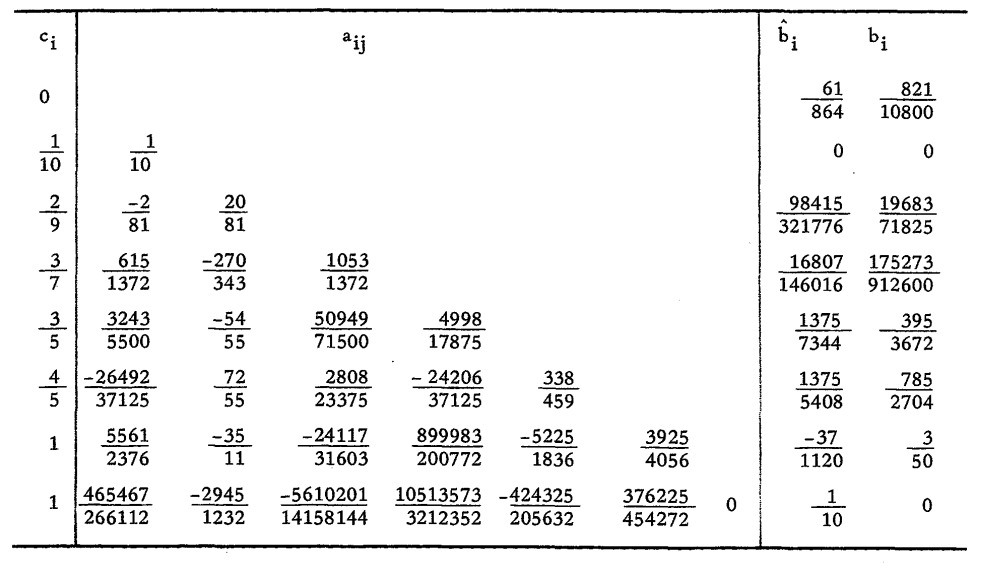
\includegraphics[width=10cm]{images/rungekutta/prdo81a}\\
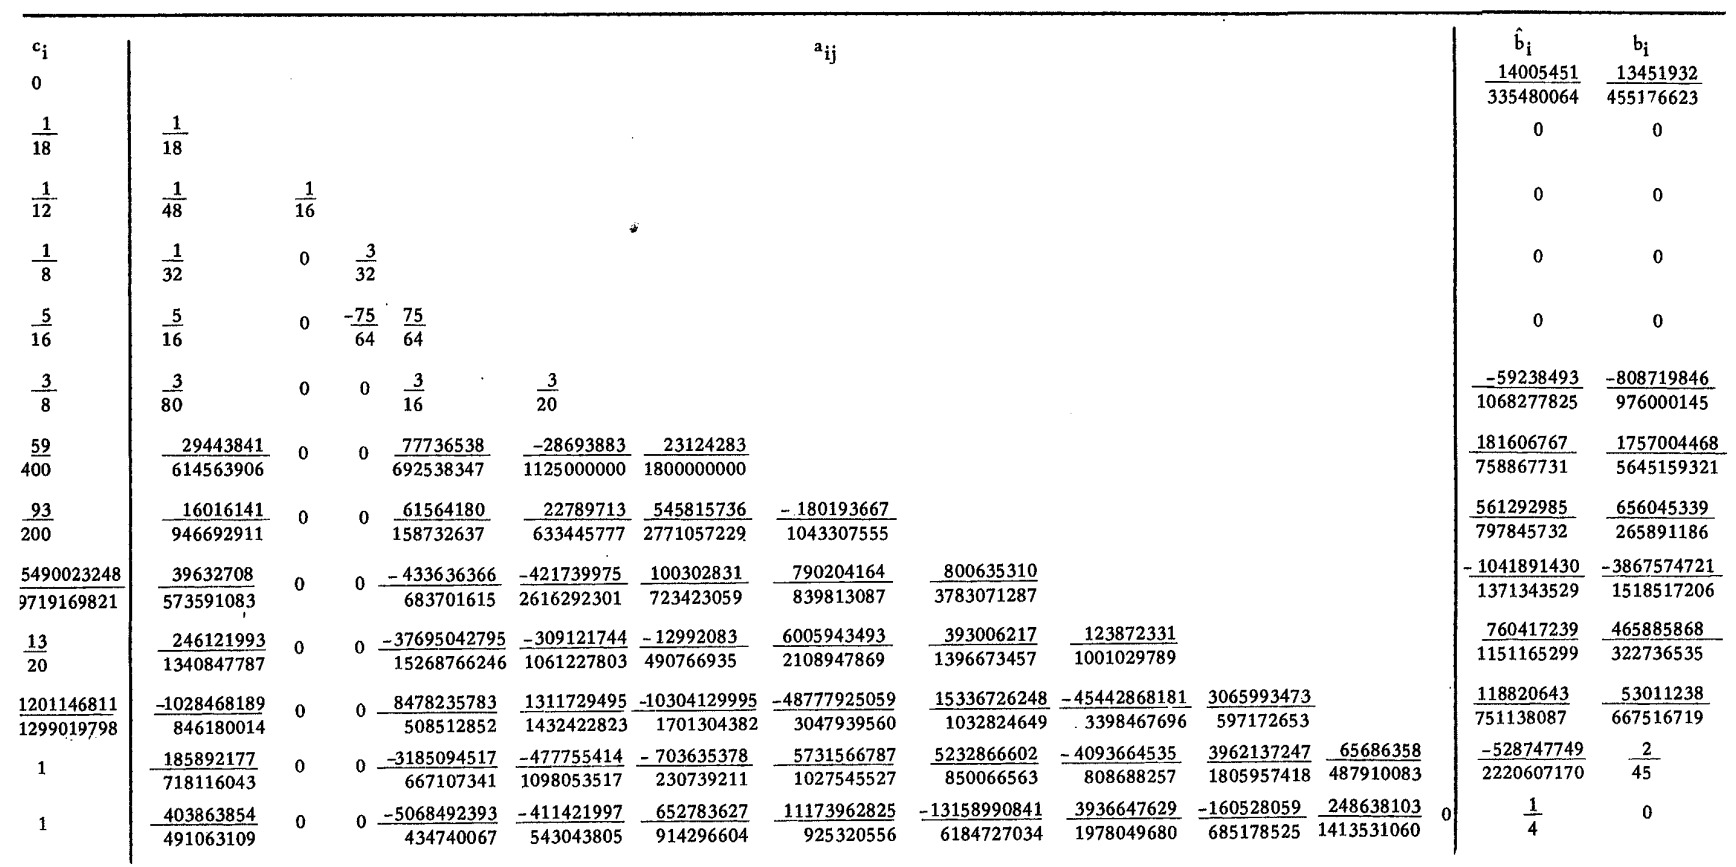
\includegraphics[width=14cm]{images/rungekutta/prdo81b}\\
{\captionfont 
RK6(5) and RK8(7) Dormand-Prince methods from \cite{prdo81}.}
\end{center}

\Literature:
\textcite{dopr80} (1980),
\textcite{fehl85} (1985),
\textcite{dopr86} (1986),
\textcite{caka90} (1990),
\textcite{hanw93} (1993),
\textcite{butcher03}.


%....................................................................................
\subsubsection{Using RK methods to advect particles/markers \label{sec:rkparticles}}

In the context of geodynamical modelling, one is usually faced with the following problem:
now that I have a velocity field on my FE (or FD) mesh, how can I use it to advect the Lagrangian 
markers?

Runge-Kutta methods are used to this effect but only their spatial component is used:
the velocity solution is not recomputed at the intermediate fractional timesteps, i.e. 
only the coefficients of the right hand side of the tableaus is used.

\begin{itemize}
\item The RK1 method is simple.

\begin{tabular}{c|c}
0 & \\
\hline
 & 1
\end{tabular}

\noindent Carry out a loop over markers and 
\begin{enumerate}
\item interpolate velocity $\vec\upnu_{m}$ onto each marker $m$
\item compute new position as follows: $\vec r_m(t+\delta t)=\vec r_m(t) + \vec\upnu_m \delta t$
\end{enumerate}

\item The RK2 method is also simple but requires a bit more work.

\begin{tabular}{c|cccccc}
0 & \\
1 & 1 \\
\hline
 & 1/2 & 1/2 
\end{tabular}

\noindent Carry out a loop over markers and 
\begin{enumerate}
\item interpolate velocity $\vec\upnu_{m}$ onto each marker $m$ at position $\vec r_m$
\item compute new intermediate position as follows: $\vec r_m^{(1)}(t+\delta t)=\vec r_m(t) + \vec\upnu_m \delta t/2$
\item compute velocity $\vec\upnu_{m}^{(1)}$ at position $\vec r_m^{(1)}$
\item compute new position: $\vec r_m(t+\delta t)=\vec r_m(t) + \vec\upnu_m^{(1)} \delta t$ 
\end{enumerate}
Note that the intermediate positions could be in a different element of the mesh so extra 
care must be taken when computing intermediate velocities. 

\item 
The RK3 method introduces two intermediate steps. 

\begin{tabular}{c|ccccc}
0 & \\
1/2 & {\color{chestnut} $\frac{1}{2}$ } \\
1 & {\color{violet}-1} & {\color{violet}2} \\ 
\hline
 & {\color{carrotorange} $\frac16$} & {\color{carrotorange} $\frac46$}  & {\color{carrotorange} $\frac16$}
\end{tabular}

Carry out a loop over markers and 
\begin{enumerate}
\item interpolate velocity $\vec\upnu_{m}$ onto each marker $m$ at position $\vec r_m$
\item compute new intermediate position as follows: 
$\vec r_m^{(1)}(t+\delta t)=\vec r_m(t) + {\color{chestnut} \frac{1}{2}} \vec\upnu_m \delta t$
\item compute velocity $\vec\upnu_{m}^{(1)}$ at position $\vec r_m^{(1)}$
\item compute new intermediate position as follows: 
$\vec r_m^{(2)}(t+\delta t)=\vec r_m(t) + ( {\color{violet}-1} \vec\upnu_m 
+ {\color{violet}2} \vec\upnu_m^{(1)} ) \delta t$
\item compute velocity $\vec\upnu_{m}^{(2)}$ at position $\vec r_m^{(2)}$
\item compute new position: 
$\vec r_m(t+\delta t)=\vec r_m(t) + ( 
{\color{carrotorange} \frac16} \vec\upnu_m + 
{\color{carrotorange} \frac46} \vec\upnu_m^{(1)} + 
{\color{carrotorange} \frac16} \vec\upnu_m^{(2)}    )\delta t$ 
\end{enumerate}

\end{itemize}

The following example is borrowed from \cite{maie12}, itself borrowed from Fullsack \cite[Section 5.4]{full95}.
It is a whirl flow \cite{otti89}, a flow with rotational symmetry in which concentric layers of material
rotate around  a centre with an angular velocity:
\[
\omega(r)= \omega_0 \frac{r}{r_0} \exp\left(-\frac{r}{r_0}  \right)
\]  
The box is $[-0.5,0.5]\times[-0.5,0.5]$, $r_0=0.25$, $\omega_0=0.3$ and $\delta t=1$. 
$60\times 60$ particles are regularly positioned inside the $[-0.3,0.3]\times[-0.3,0.3]$ square.
Maierova \cite{maie12} has carried out this experiment for the above Runge-Kutta methods.

\begin{center}
\includegraphics[height=4cm]{images/rk/maie12a}\\
{\captionfont Model domain with particles colored at three
different time-steps: (A) t = 0 (initial position of particles), (B) t = 50, and (C) t = 200.
The advection is computed using the fourth-order Runge-Kutta scheme. Taken from \cite{maie12}}
\end{center}

\begin{center}
\includegraphics[height=4cm]{images/rk/maie12b}
\includegraphics[height=4cm]{images/rk/maie12c}\\
{\captionfont The same plot as above, but for different advection schemes at t = 100.
Advection was computed using (A) the fourth-order Runge-Kutta scheme, (B) the mid-
point method, (C) Heun's method and (D) the explicit Euler method. Taken from \cite{maie12}}
\end{center}


